\section{Pistepilven visualisointi sisäkkäispistepuilla}\label{mun}

Luvussa \ref{usecase} todettiin Scheiblauerin ja Schützin ehdottamien sisäkkäispistepuiden soveltuvan laitossuunnitteluohjelmistossa käytettävän pistepilvivisualisoijan tarpeisiin. Sisäkkäispistepuiden rakenne mahdollistaa seuraavaksi esiteltävän yksinkertaisen tekniikan pistedatan kompressioon. Tämän jälkeen esitellään algoritmeja sisäkkäispistepuun rakentamiseen, renderöintiin ja pisteiden valitsemiseen.

\subsection{Pistedatan esitysmuoto}\label{kompressio}

Pistepilvet sisältävät usein satoja miljoonia tai jopa miljardeja pisteitä, mikä johtaa luonnollisesti isoihin tiedostokokoihin. Yleensä hierarkiatiedon osuus tiedoston sisällöstä on varsin pieni, joten tiedostokokoa saadaan pienennettyä parhaiten tiivistämällä itse pisteiden esitysmuotoa. Pisteistä tarvitsee tallentaa vähintään niiden sijainti ja väri. Yleensä sijainti esitetään kolmella nelitavuisella liukuluvuilla ja väri RGB-koodauksella kolmella tavulla:

\code{
struct Point \{\\
    \tab float x;\\
    \tab float y;\\
    \tab float z;\\
    \tab unsigned char r;\\
    \tab unsigned char g;\\
    \tab unsigned char b;\\
    \}
}

\noindent Yleensä näiden 15:a tavun lisäksi lisätään yksi pakkaustavu, jotta koko olisi mukava kahden potenssi. Miljardi pistettä tallennettuna tässä esitysmuodossa vaatisi siis 16 gigatavua muistia. Muuttamalla pisteiden esitysmuotoa voidaan pistepilviä tiivistää ja joitakin operaatioita nopeuttaa.

\begin{figure}
    \subfile{fig/ruudukko.tex}
    \caption{64:n solun ruudukko, jonka indeksointi alkaa vasemmasta alakulmasta}
    \label{ruudukkokuva}
\end{figure}

Puun rakennusvaiheessa pisteet lisätään jokaisessa solmussa olevaan kolmiulotteiseen ruudukkoon, jonka jokaiseen soluun mahtuu vain yksi piste. Kun piste lisätään ruudukon soluun, tallennetaan solun järjestysnumero hajautustauluun, josta voidaan jatkossa nopeasti tarkastaa, onko kyseinen solu varattu. Mahdollinen numerointi ruudukolle on esitetty kuvassa \ref{ruudukkokuva}. Numerointi alkaa vasemmasta alakulmasta indeksistä nolla ja etenee vasenkätisen koordinaatiston mukaisesti. 

Sisäkkäispistepuiden käyttämä ruudukko mahdollistaa yksinkertaisen pakkausalgoritmin. Puun solmuihin on tallennettu rajauslaatikko, joka määrittää myös ruudukon mitat ja sijainnin. Ruudukkoon lisättävien pisteiden absoluuttinen sijainti voidaan unohtaa ja käyttää sijainnin tallentamiseen pisteen suhteellista sijaintia ruudukossa. Yksinkertaisimmillaan voidaan kustakin pisteestä tallentaa vain sen solun indeksi, jossa piste sijaitsee. Tällöin pisteen esitysmuoto on siis

\code{
struct Point \{\\
    \tab unsigned int index;\\
    \tab unsigned char r;\\
    \tab unsigned char g;\\
    \tab unsigned char b;\\
    \}
}

\noindent Kun solun indeksi tallennetaan etumerkittömänä nelitavuisena kokonaislukuna ja lisätään loppuun yksi pakkaustavu, tiivistyy piste kahdeksantavuiseksi. Näin miljardi pistettä vaatisi enää 8 gigatavua muistia. 

Esitysmuotoa voidaan tiivistää vielä tästäkin. Pisteen etäisyyttä suhteessa ruudukkoon voidaan esittää kolmella tavulla niin, että jokainen tavu kuvaa koordinaattiakselien suuntaisten askelten määrää ruudusta 0 lähtien. Yhden tavun esittämä enimmäisarvo on 255, joten ruudukossa voi olla enintään $255^3=16581375$ solua. Tällainen kompressio tuo toki pistepilveen epätarkkuutta, johon palataan pian.

Usein laitossuunnittelussa käytetyissä laserkeilaimissa ei käytetä värikameraa antamaan pisteille värejä, vaan väri-informaatio johdetaan keilaimeen heijastuvan valon määrästä. Tämä arvo normalisoidaan yleensä välille $[0,255]$, josta saadaan jokin harmaan sävy. Tällaisissa pistepilvissä on siis turha tallentaa jokaiselle pisteelle \texttt{r}, \texttt{g} ja \texttt{b} -arvoja, kun vain yksi arvo riittäisi. Näin piste voidaan esittää muodossa 

\code{
struct Point \{\\
    \tab unsigned char dx;\\
    \tab unsigned char dy;\\
    \tab unsigned char dz;\\
    \tab unsigned char intensity;\\
    \}
}

\noindent eli tarvitaan vain neljä tavua tilaa ja edellä mainittu pistepilvi saadaan tiivistettyä neljännekseen alkuperäisestä koostaan. 

\begin{figure}
    \centering
    \subfile{fig/error.tex}
    \caption{Suurin mahdollinen ruudukossa esiintyvä virhe $\epsilon$. Kuutio kuvaa ruudukon solua ja asteriski sen visualisointiin käytettävää keskipistettä. Soluun lisätty punainen piste on juuri ja juuri solun sisällä.}
    \label{errorkuva}
\end{figure}

Kun pisteen tarkka sijainti unohdetaan ja se ilmaistaan suhteessa ruudukkoon, syntyy pistepilveen virheitä. Suurinta mahdollista virhettä on havainnollistettu kuvassa \ref{errorkuva}, kun piste visualisoidaan solun keskipisteenä, vaikka se oikeasti sijaitsisi aivan sen nurkassa. Jos oletetaan, että ruudukon solut ovat kuutioita, saadaan enimmäisvirhe laskettua helposti Pythagoraan lauseella muotoon 
\begin{equation}
    \epsilon = \frac{a \sqrt{3}}{2}.      
\end{equation}

Vaatimus \ref{vaatimus:virhe} esitti virheen enimmäissuuruudeksi yhtä millimetriä. Oktettipuu jakaa rajauslaatikon sivun kahtia joka tasolla ja ruudukko sen edelleen pieniin soluihin. Jos oletetaan esimerkiksi pistepilven rajauslaatikko kuutioksi, jonka sivun pituus on sata metriä ja ruudukon sisältävän Scheiblauerin ja Schützin käyttämää 128 solua jokaiseen koordinaattiakselin suuntaan, saavutetaan puun tasolla 11 ruudukko, jonka solun sivun pituus on $a = \frac{100m/2^{10}}{128} \approx 0,763mm$. Tällaisessa ruudukossa enimmäisvirhe on $\frac{0,763mm \cdot \sqrt{3}}{2} \approx 0,661mm$, joten kaikki tähän ruudukkoon lisätyt pisteet täyttävät vaatimuksen \ref{vaatimus:virhe}. Tämä ei tarkoita sitä, että puu voisi sisältää pisteitä vain tasolle 11 ja sitä syvemmälle. Pisteitä voi hyväksyä suuriinkin soluihin, jos ne ovat sattuvat osumaan tarpeeksi lähelle sen keskipistettä. Käytännössä suurissa pistepilvissä on pisteitä yleensä niin tiheästi, että puun ylimmillekin tasoille tulee tallennetuksi pisteitä.

Pisteiden sijainnin suhteellinen esitysmuoto nopeuttaa myös pistepilvien käsittelyä. Laitossuunnittelussa pistepilveä joudutaan usein sovellukseen latauksen jälkeen liikuttamaan ja skaalaamaan, jotta se istuisi hyvin 3d-malliin. Jos pisteisiin olisi tallennettu absoluuttinen sijainti, jouduttaisiin pistepilveä tallennettaessa uudelleenkirjoittamaan kaikki pisteet käyttäjän määrittämällä transformaatiomatriisilla kerrottuna. Edellä kuvatulla esitysmuodolla transformaatio täytyy suorittaa vain oktettipuun solmujen rajauslaatikoilla, joista tiivistetyn pisteen sijainti johdetaan. Tämä johtaa merkittävään parannukseen käyttökokemuksessa, sillä satojen miljoonien pisteiden kirjoittaminen levylle kestää useita minuutteja.

\subsection{Tietorakenteen rakentaminen}

%Edellä todettiin sisäkkäispistepuiden sopivan pistepilvien käsittelyyn käytettäväksi tietorakenteeksi laitossuunnitteluohjelmistossa ja ehdotettiin pisteille kompaktimpaa esitysmuotoa. Käydään nyt läpi puun rakentamiseen käytettyjä algoritmeja.

Edellä esitellyn oktettipuun rakentaminen suoritetaan kahdessa vaiheessa. Ensin käydään kaikki syötepisteet läpi ja selvitetään niille rajauslaatikko. Tämän jälkeen luodaan tyhjä juurisolmu, jonka rajauslaatikkona toimii äsken laskettu, kaikki pisteet sisältävä tila. Nyt syötepisteet voidaan lisätä yksitellen juurisolmuun, joka syöttää ne tarvittaessa edelleen lapsisolmuilleen. Rakentamisen ylintä tasoa on kuvattu algoritmissa \ref{alg:rakenna}.

\begin{algorithm}[!h]
    \caption{RakennaOktettipuu}
    \label{alg:rakenna}
    \subfile{alg/rakennapuu.tex}
\end{algorithm}

Algoritmi \ref{alg:lisaaPiste} huolehtii pisteen pisteen lisäämisestä solmuun. Piste hyväksytään solmuun, jos sitä vastaava ruudukon solu on tyhjä, sen etäisyys solun keskipisteestä on pienempi kuin sallittu enimmäisvirhe ja solussa ei ole jo liikaa pisteitä. Solmujen sisältämien pisteiden määrälle kannattaa asettaa yläraja, jotta saavutettaisiin sopiva haarautuminen.

Puun syvyyttä voi rajoittaa asettamalla ruudukon soluille vähimmäismitat. Yleensä laserkeilaimen lähellä olevat pinnat tulevat näytteistetyksi hyvin tiheästi ja tilannetta pahentaa, jos useat keilaimet ovat mitanneet samoja pintoja tiheästi. Algoritmin \ref{alg:lisaaPiste} rivillä 3 tarkastetaan, ylittäisikö uusi lapsisolmu puun enimmäissyvyyden. Kun ennaltamäärätylle pohjatasolle hyväksytään kaikki pisteet, kunhan niitä vastaava ruudukon solu on vapaa, saadaan pistepilvelle tehokas ja globaali enimmäistiheys. Tällä tavalla pilveä saadaan harvennettua tehokkaasti ja vaatimus \ref{vaatimus:harvennus} voidaan tyydyttää. %TODO: \ref{arviointi} missä tätä toivottavasti on mitattu

\begin{algorithm}[!h]
    \caption{LisääPisteSolmuun}
    \label{alg:lisaaPiste}
    \subfile{alg/lisaaPiste.tex}
\end{algorithm}

Jotta säästettäisiin satojen tuhansien tiedostojen avaamisen ja sulkemisen vaatima aika, voidaan laitossuunnitteluohjelmistossa tietorakenne tallentaa yhteen tiedostoon. Tallennettaessa kirjoitetaan tiedostoon ensin tarvittavat tiedot puun solmuista ja pisteet vasta niiden jälkeen. Jokainen solmu sisältää tiedon siitä, kuinka monta pistettä siihen kuuluu, sekä ensimmäisen pisteen indeksin pistetaulukossa. Tämä mahdollistaa sen, että pistepilveä käsiteltäessä luetaan tiedostosta ensin vain kevyt hierarkia, jonka jälkeen vain tarvittavat pisteet voidaan lukea muistiin. Tiedoston rakennetta on havainnollistettu kuvassa \ref{layout}. Pisteiden lukumäärän ja ensimmäisen pisteen indeksin lisäksi jokaisesta solmusta tallennetaan rajauslaatikko ja sijaintikoodi, joka kertoo sen sijainnin puussa. Sijaintikoodin  numerot kertovat reitin juurisolmusta kyseiseen solmuun. Esimerkiksi koodi 014 tarkoittaa juurisolmun toisessa oktetissa sijaitsevan lapsen viidennessä oktetissa sijaitsevaa lasta. Lopuksi tarvitsee levylle kirjoittaa vielä millä puun tasolla se sijaitsee, jotta tiedostoa lukiessa tiedettäisiin sijaintikoodin pituus.

\begin{figure}
    \centering
    \subfile{fig/layout.tex}
    \caption{Tiedostoon tallennetaan ensin puun solmut, joiden jälkeen kaikki pisteet ovat peräkkäin taulukossa. Punaiset nuolet kuvaavat solmuihin tallennettuja indeksejä pistetaulukkoon, josta siihen kuuluvat pisteet alkavat.}
    \label{layout}
\end{figure}

Yksittäinen solmu voidaan siis kirjoittaa levylle muodossa 

\code{
struct Node \{\\
    \tab float min\_x;\\
    \tab float min\_y;\\
    \tab float min\_z;\\
    \tab float max\_x;\\
    \tab float max\_y;\\
    \tab float max\_z;\\
    \tab unsigned char depth;\\
    \tab unsigned char location\_code[];\\
    \tab unsigned int num\_points;\\
    \tab unsigned int point\_index;\\
    \}
}

\noindent Nelitavuisilla liukuluvuilla ja kokonaisluvuilla vaatii solmu siis tallennustilaa $33 + d$ tavua, missä $d$ on solmun syvyys puussa.

Edellä kuvattu rakennusalgoritmi pitää koko oktettipuun muistissa ennen kuin pisteet kirjoitetaan levylle. Massiivisten pistepilvien tapauksessa keskusmuisti saattaa täyttyä vaikka pilveä olisi harvennettu ja pisteitä kompressoitu. Muisin täyttyessä käyttöjärjestelmä alkaa pitää osaa prosessin muistiavaruudesta kiintolevyllä sivutuksen \engl{paging} avulla \cite{os}. Jatkotutkimuksen aiheeksi jää selvittää, onko nopeampaa antaa käyttöjärjestelmän siirtää sivuja kiintolevylle, vai esimerkiksi tallentaa ensin pisteitä väliaikaisiin tiedostoihin niiden lisäysjärjestykessä, josta ne kopioidaan oikeassa järjestyksessä lopulliseen tiedostoon. 

\subsection{Visualisointi}\label{render}

Nopein tapa visualisoida pistepilvi on pitää kaikki pisteet näytönohjaimen muistissa ja joka ruudunpäivityksellä piirtää kaikki näkymässä näkyvät pisteet. Vaikka koko pistepilvi mahtuisi näytönohjaimen muistiin, täytyy laitossuunnitteluohjelmistossa visualisoida muutakin grafiikkaa. Näytönohjaimen muistia voidaan säästää käyttämällä niin kutsuttua puskurivirtaa \engl{buffer streaming}. Yleinen ongelma grafiikan piirtämisessä on se, että näytönohjain prosessoi dataa nopeammin kuin suoritin ehtii sille syöttää. Puskurivirran ajatuksena on pitää näytönohjain mahdollisimman toimeliaana jakamalla puskuri, jonka kautta dataa siirretään keskusmuistista näytönohjaimen muistiin, kolmeen osaan. Samalla kun näytönohjain käsittelee yhtä puskurin osaa, suoritin voi täyttää toista datalla, ja kolmas on jo palautumassa suorittimen täytettäväksi. Teoriassa näytönohjain voi vain vaihtaa luettavaa osiota ilman, että sen tarvitsisi odottaa lainkaan hidasta tiedonsiirtoa. \cite{opengl}

\begin{figure}
    \centering
    \subfile{fig/triplebuffering.tex}
    \caption{Pistedatan visualisoinnissa käytetty puskuri, joka on jaettu osioihin $b_0$, $b_1$ ja $b_2$. Osioon $b_0$ on kirjoitettu pisteet solmuista $s_0$-$s_3$. Puskurivirran tarkoituksena on vähentää tiedonsiirrosta aiheutuvaa latenssia.}
    \label{triplebuffering}
\end{figure}

Kuvassa \ref{triplebuffering} pistepuskuri on jaettu osioihin $b_0$, $b_1$ ja $b_2$. Puskurin koko on valittu niin, että jokaiseen osioon mahtuu neljän täyden solmun pisteet. Käytännössä solmut eivät kuitenkaan aina ole täysiä, joten on mahdollista, että osiot jäävät vajaiksi. Puskureita kuitenkin vaihdetaan tiuhaan, joten ei ole järkevää käyttää aikaa puskurin täyttöasteen maksimointiin.

Tietorakenteen visualisointia testatessa puskurivirta ei kuitenkaan tuottanut tarpeeksi miellyttävää visuaalista lopputulosta. Etenkin pilveä pyöriteltäessä ja sen läpi liikuttaessa puskurivirralla ehdittiin pilvestä piirtää vain hyvin karkea tarkkuus niin, että ruudunpäivitystaajuus pysyi interaktiivisena. Ratkaisuna tähän näytti toimivan hyvin Futterliebin et al. \cite{smooth} innoittamana toinen pistepuskuri, jossa säilytetään karkeaa yleiskuvaa pilvestä. Tämä yleiskuvapuskuri pidetään näytönohjaimen muistissa, josta se on nopea piirtää jokaisella ruudunpäivityksellä. 

\begin{algorithm}[!h]
    \caption{PiirräSisäkkäispistepuu}
    \label{alg:render}
    \subfile{alg/render.tex}
\end{algorithm}

Algoritmissa \ref{alg:render} yleiskuvapuskuri täytetään ensimmäisellä visualisointikerralla puun ylimpien tasojen solmujen pisteillä, jotka muodostavat karkean, mutta kattavan yleiskuvan pilvestä. Yleiskuvapuskurista voisi yrittää vaihtaa näkymän ulkopuolella olevia pisteitä näkyviin solmuihin, mutta näkyvyystarkastelun suorittaminen ja puskurin muokkaaminen jokaisella ruudunpäivityksellä osoittautui liian aikaavieväksi. 
%Seuraavilla renderöintikerroilla puskurista tarkistetaan, ovatko niiden sisältämät pisteet vielä näkyvissä. Jokaista pistettä ei tarvitse tarkastaa, jos ylläpidetään listaa solmuista, joiden pisteet puskuriin lisättiin. Jos näkymä on muuttunut niin, että jokin solmu ei enää ole näkyvissä, vaihdetaan sen pisteet toisen solmun pisteisiin. Yleiskuvapuskurissa pidetään solmuja mahdollisimman läheltä puun juurta, jotta ne muodostaisivat tarpeeksi kattavan kuvan koko pistepilvestä.

\begin{algorithm}[!h]
    \caption{PiirräPuskurivirta}
    \label{alg:renderDetail}
    \subfile{alg/renderDetail.tex}
\end{algorithm}

Yleiskuvan visualisoinnin jälkeen jäljelle jäävät solmut järjestetään niiden kuvaruudulle projisoidun koon mukaan, koska kuva näyttää tarkentuvan nopeammin, kun ensin piirretään suuret ja lähellä kameraa olevat solmut. Järjestämisen jälkeen loput pisteet voidaan piirtää algoritmissa \ref{alg:renderDetail} kuvatulla puskurivirralla. 

Algoritmi \ref{alg:renderDetail} lisää kunkin solmun pisteet täyttövuorossa olevaan puskurivirran osioon. Puskuriosion täyttyessä vaihdetaan täytettäväksi seuraava osio. Puskurivirtaa käyttäessä täytyy varmistaa, ettei sama osio ole sekä suorittimen kirjoitettavana, että näytönohjaimen luettavana. Tämä tapahtuu lähettämällä näytönohjaimelle jokaisen puskuriosion täyttymisen jälkeen synkronointiobjekti \engl{sync object}. Kun uutta osiota otetaan kirjoitettavaksi, tarkastetaan, että näytönohjain on merkannut kyseisen osion synkronointiobjektin käsitellyksi. \cite{sync}

Algoritmi \ref{alg:render} suorittaa pistepilvelle näkyvyyskarsintaa \engl{visibility culling} valitessaan rivillä 11 visualisoitavaksi vain ne solmut jotka ovat täysin tai osittain näkymäkartion \engl{view frustum} sisällä. Näkyvyyskarsinnan lisäksi algoritmin voidaan katsoa suorittavan yksinkertaista yksityiskohtien karsintaa \engl{detail culling}, kun kuvaruudulle suurena projisoidut solmut visualisoidaan ensin.

Yksityiskohtien karsinta on suosittu nopeutustekniikka tietokonegrafiikassa. Ajatuksena on visualisoida vain tärkeimmät objektit ja jättää kaukana olevat tai pienet objektit käsittelemättä, jotta ruudunpäivitystaajuus pysyy interaktiivisena. Yksinkertainen tapa karsia yksityiskohtia on järjestää objektit niiden kuvaruudulle projisoidun koon mukaan ja piirtää niitä tiettyyn rajaan asti, tai kunnes aika loppuu kesken. Akenine-Möller et al. \cite{rrr} esittävät kuvaruudulle projisoidun objektin koon arviolle kaavaa 
\begin{equation}
    a = \pi (\frac{nr}{\mathbf{d} \cdot (\mathbf{c}-\mathbf{v})})^2,
\end{equation} jossa $n$ on katselupisteen etäisyys kuvatasosta, $r$ objektin rajauspallon säde ja $\mathbf{c}$ keskipiste, $\mathbf{d}$ on normalisoitu katsomissuunta, ja $\mathbf{v}$ katselupiste. \cite{mikko}

Mikko Yllikäinen huomautti pro gradu -tutkielmassaan \cite{mikko}, ettei tarkkaa arvioita objektien koosta kannata selvittää, jos halutaan selville vain suuruusjärjestys. Yllikäinen yksinkertaistaa kaavan muotoon 
\begin{equation}
    \begin{split}
    a & = \frac{r}{\mathbf{d} \cdot ( \mathbf{c} - \mathbf{v} )}\\
    & \approx \frac{r}{\sqrt{(c_x-v_x)^2 + (c_y-v_y)^2 + (c_z - v_z)^2}}\\
    & \propto \frac{r}{(c_x-v_x)^2 + (c_y-v_y)^2 + (c_z - v_z)^2}.    
    \end{split}
\end{equation}
 Yllikäinen nimittää tällä kaavalla muodostetu suuruusjärjestyksen käyttämistä yksityiskohtien karsinnassa kontribuutiokarsinnaksi \engl{contribution culling}. On huomattava, että tällainen karsinta ei ole mahdollista paralleliprojektiomaisemissa, joissa katseluetäisyys ei vaikuta objektien kokoon. \cite{mikko}


\subsection{Pisteiden valitseminen}

Yksittäisten pisteiden valitseminen pistepilvestä on hyvin raskas operaatio, jos pisteet eivät ole hierarkisessa tietorakenteessa. Oktettipuuta käytettäessä kaikkia pisteitä ei tarvitse kuitenkaan käydä läpi. Käyttäjän valitessa hiirellä piste ammutaan kamerasta säde kursorin projisoidun sijainnin läpi pistepilveen. Nyt pisteitä tarvitsee etsiä vain niistä oktettipuun solmuista, joihin säde osuu. Yksinkertaisimmillaan voidaan valita sädettä lähinnä oleva piste. Tällöin valituksi saattaisi kuitenkin tulla muukalaispiste, joka sattuu olemaan juuri kameran edessä. Yksinkertainen tapa välttää muukalaispisteen valitsemista olisi hylätä sellaiset puun solmut, joissa säde osuu vain yhteen tai muutamaan pisteeseen. Toinen vaihtoehto olisi kerätä useita kandidaattipisteitä ja hylätä varmuuden vuoksi muutama kursoria lähinnä oleva piste.

%\begin{figure}
%    \centering
%    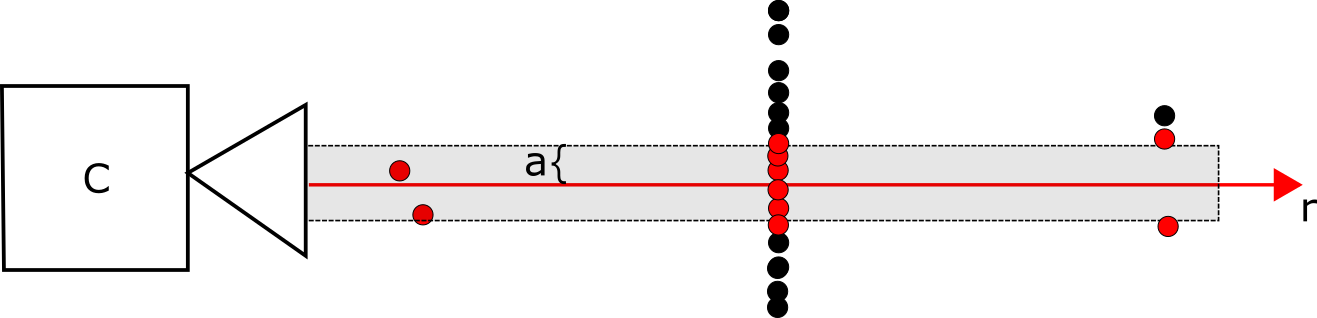
\includegraphics[width=\textwidth]{img/shootRay}
%    \caption{Piste valitaan pilvestä ampumalla säde $r$ kamerasta $C$ maisemaan. $a$- säteisen lieriön sisäpuolella olevista, punaisella merkatuista pisteistä jokin on käyttäjän haluama piste.} 
%    \label{img:ray}
%\end{figure}

%Jotta voitaisiin välttää väärien pisteiden valitseminen vahingossa, kannattaa säteen läheltä ensin kerätä useampi potentiaalinen piste, joista lopullinen valintapiste valitaan. Kuvassa \ref{img:ray} on esitetty kamerasta $C$ lähtevä säde $r$, jonka ympärillä on $a$-säteinen lieriö. Kaikki lieriön sisäpuolella olevat pisteet valitaan jatkokäsiteltäväksi. Yksinkertainen, mutta käytännössä toimivaksi todettu tapa hylätä ei-toivotut pisteet potentiaalisisten pisteiden joukosta on järjestää pisteet niiden kamerasta katsotun etäisyyden perusteella ja jättää pois lähin ja kauimmaisin kolmasosa. Jäljelle jääneistä pisteistä valitaan se, joka on lähinnä sädettä.

Oktettipuun rakenne auttaa myös vaatimuksen \ref{vaatimus:crop} tyydyttämisessä. Jos pistepilvestä halutaan piilottaa tai korostaa tiettyä osaa, voi käyttäjä valita maisemasta laatikon ja muokata sen sisältämien pisteiden näkyvyyttä. Oktettipuuta käytettäessä ei jokaisen pisteen sisältymistä valintalaatikoihin tarvitse selvittää, vaan riittää tarkastaa, onko solmun rajauslaatikko valintalaatikon sisällä. Vain siinä tapauksessa, että rajauslaatikko on vain osittain valintalaatikon sisällä, tarvitsee tarkastus tehdä kaikille pisteille. Valintalaatikoita voidaan pitää muistissa visualisointivaiheessa ja jokaisen solmun kohdalla tarkistaa sen sisältyvyys valintalaatikoihin.

Scheiblauer esittää väitöskirjassaan sisäkkäisille muokattaville oktettipuille erityistä tietorakennetta valittujen pisteiden käsittelyyn. Scheiblauer valitsee pisteitä puusta laatikkovalitsimella tai kolmiulotteisella siveltimellä \engl{volumetric brush}, ja lisää ne erityiseen valintaoktettipuuhun \engl{selection octree}. Kun halutut pisteet on valittu, kuvaa valintaoktettipuu valittujen pisteiden asuttamaa avaruuden osaa. Valintaoktettipuuta käytetään esimerkiksi pisteiden piilottamiseen näkymästä. Pisteitä piirrettäessä tarkastetaan, osuuko sen sijainti valintaoktettipuun solmuihin ja päätetään sen perusteella, hylätäänkö piste vai ei. \cite{scheiblauer}

Alustavien tulosten perusteella pisteiden valinta oli riittävän nopeaa ilman Scheiblauerin ehdottamia valintaoktettipuita. Jatkotutkimuksen aiheeksi jää selvittää, minkälainen ero suorituskyvyssä on edellä esitetyn, yksinkertaisen valintatekniikan ja valintaoktettipuiden välillä.